\labeledsection{Natural Language Processing}{sec:nlp}
\anondefinition{
\defemph{Natural Language Processing (NLP)} is an engineering field at the intersection of computer science, AI, and linguistics which is concerned with the interactions between computers and human (natural) languages. Most challenges in \defemph{NLP} involve:
\begin{itemize}
    \item \defemph{Natural Language Understanding (NLU)}: enabling computers to derive meaning (\linkterm{representations}{representation}) from human or \linkterm{natural language}{natural_language} input.
    \item \defemph{Natural Language Generation (NLG)}: enabling computers to generate \linkterm{natural language}{natural_language} or speech from those \linkterm{representations}{representation}.
\end{itemize}
}{NLP}

\commandnote{
We need both \linkterm{NLU}{NLP} and \linkterm{NLG}{NLP}
}

\anondefinition{
We say that a symbol or expression $e$ \defemph{represents} a concept, object, or \linkterm{proposition}{proposition} $M$ if the meaning of $e$ is $M$.
}{representation}

\anondefinition{
An \defemph{utterance} is the smallest unit of speech. It is a continuous piece of speech beginning and ending with a clear pause. \linkterm{Representations}{representation} of \defemph{utterances} in written \linkterm{natural language}{natural_language} are called \defemph{natural language utterances}.
}{utterance}


\centeredtitledbox{Interpretation of \linkterm{natural language utterances}{utterance} - Three problems}{
\anondefinition{
\defemph{abstraction} refers to the phenomenon where multiple distinct natural language expressions or words point to a single, identical meaning or representation (e.g., synonyms like "car" and "automobile" mapping to the same underlying concept).
}{abstraction}

\anondefinition{
\defemph{ambiguity} occurs when a single natural language expression or word maps to multiple distinct meanings or representations (e.g., the word "bank" referring to either a financial institution or a geographical feature).
}{ambiguity}

\anondefinition{
\defemph{composition} (or \defemph{compositionality}) refers to the principle where the meaning of a complex expression is determined by the individual meanings of its parts and the rules used to combine them, allowing for systematic mapping to structured formal representations (e.g., evaluating "Every student sleeps" as $\forall x.student(x) \Rightarrow sleep(x)$).
}{composition}
}

\begin{figure}[H]
    \centering
    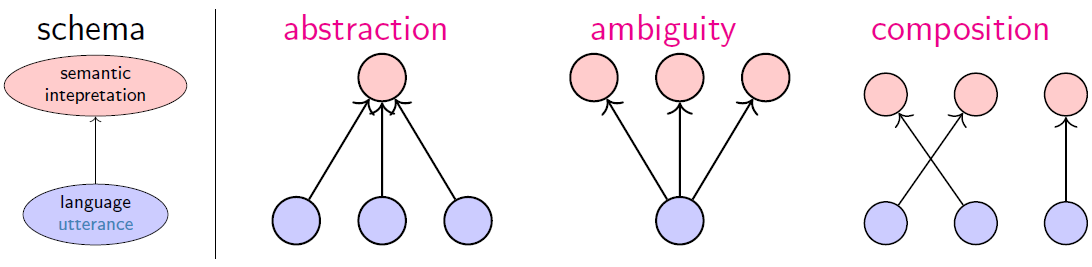
\includegraphics[width=0.5\linewidth]{images/nlp_problems.png}
\end{figure}

\commandnote{
While formal semantics assumes that the meaning of an utterance is a strict function of its parts and its syntax, natural language frequently violates this principle through idioms, metaphors, and conventionalized phrases. An interpreter cannot rely solely on a universal set of composition rules and must instead maintain a massive, dynamic lexicon of multi-word expressions.
}

\anondefinition{
We call a piece $i$ of information \defemph{linguistically realized} in an \linkterm{utterance}{utterance} $U$, iff we can trace $i$ to a fragment of $U$.
}{linguistically_realized}

\problembox{
Not all information conveyed is \linkterm{linguistically realized}{linguistically_realized} in an \linkterm{utterance}{utterance}.

\Example{
\textit{"The lecture begins at 11:00 am"} \hfill{What lecture? Today?}
}{}
}

\anondefinition{
\defemph{Semantic / Pragmatic Analysis} is a possible mechanism to infer the missing pieces from the context and world knowledge.

\begin{figure}[H]
    \centering
    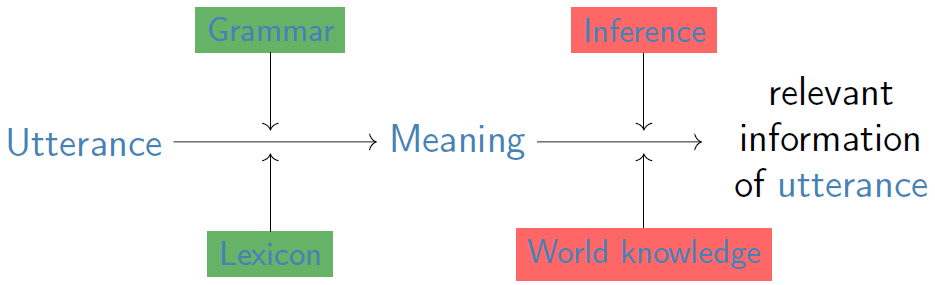
\includegraphics[width=0.5\linewidth]{images/semantic-analysis.png}
\end{figure}
}{semantic_analysis}

\problembox{
Sometimes, more inference is needed. e.g. \textit{"It starts at eleven"}. Before we resolve time, we need to resolve \textit{"it"}.
}

\begin{figure}[H]
    \centering
    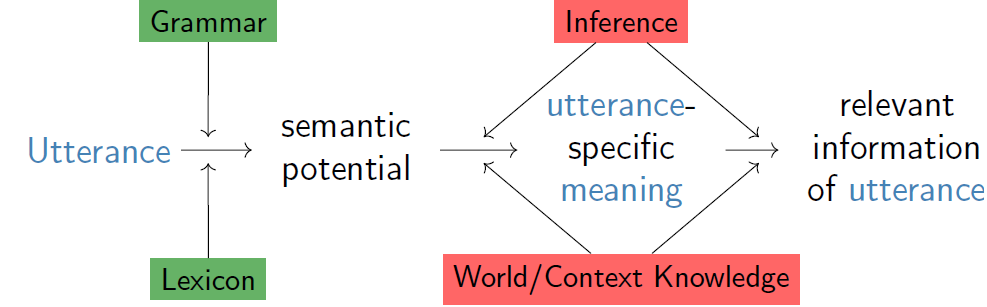
\includegraphics[width=0.5\linewidth]{images/nl_more_infer.png}
\end{figure}

\definition{Readings}{
We call an \linkterm{utterance}{utterance} ambiguous, iff it has multiple \linkterm{representations}{representation} (meanings), which we call \defemph{readings}
}{readings}


\Example{
\textbf{Lexical Ambiguity:}

The utterance \textit{"I went to the bank"} yields two distinct \linkterm{readings}{readings} based on lexical ambiguity:
\begin{itemize}
    \item \textbf{Reading 1:} $\text{go\_to}(\text{me}, \text{financial\_institution})$
    \item \textbf{Reading 2:} $\text{go\_to}(\text{me}, \text{river\_bank})$
\end{itemize}
}{}

\Example{
\textbf{Syntactic Ambiguity:}

The utterance \textit{"I saw the man with the telescope"} yields two distinct \linkterm{readings}{readings} based on structural attachment:
\begin{itemize}
    \item \textbf{Reading 1 (Instrumental):} $\text{see}(\text{me}, \text{man}) \wedge \text{use}(\text{me}, \text{telescope})$ 
    \item \textbf{Reading 2 (Modifier):} $\exists x. \text{man}(x) \wedge \text{see}(\text{me}, x) \wedge \text{has}(x, \text{telescope})$
\end{itemize}
}{}

\anondefinition{
A word or phrase is called \defemph{anaphoric} (or an \defemph{anaphor}) if its interpretation depends upon an earlier phrase in the context, which is called its \defemph{antecedent}.
}{anaphor}

\Example{
\textit{"Jane lost her keys, and she couldn't find them"}
\begin{itemize}
    \item \linkterm{anaphor}{anaphor} \textit{"she"} refers to \linkterm{antecedent}{anaphor} \textit{"Jane"}
    \item \linkterm{anaphor}{anaphor} \textit{"them"} refers to \linkterm{antecedent}{anaphor} \textit{"keys"}
\end{itemize}
}{}

\anondefinition{
A word or phrase is called \defemph{cataphoric} (or a \defemph{cataphor}) if its interpretation depends upon a later phrase in the context, which is called its \defemph{postcedent}.
}{cataphor}

\Example{
\textit{"Because he was late, John missed the bus"}
\begin{itemize}
    \item \linkterm{cataphor}{cataphor} \textit{"he"} refers to \linkterm{postcedent}{cataphor} \textit{"John"}
\end{itemize}
}{}

\commandnote{
We sometimes say \refterm{anaphoric phrase}{anaphoric_phrase} to mean \linkterm{anaphor}{anaphor} or \linkterm{cataphor}{cataphor}
}

\anondefinition{
The process of determining the \linkterm{antecedent}{anaphor} or \linkterm{postcedent}{cataphor} of an \linkterm{anaphoric phrase}{anaphoric_phrase} is called \defemph{anaphor resolution} or \defemph{anaphoric resolution}
}{anaphor_resolution}

\anondefinition{
An \linkterm{anaphoric}{anaphoric_phrase} connection between \linkterm{anaphor}{anaphor} and its \linkterm{antecedent}{anaphor} or \linkterm{postcedent}{cataphor} is called \defemph{direct}, iff it can be understood purely \linkterm{syntactically}{syntactic_analysis_grammar}.
}{direct_anaphoric_conn}

\Example{
\textit{"Sarah ate the apple. She found it delicious"}
}{}

\anondefinition{
An \linkterm{anaphoric}{anaphoric_phrase} connection between \linkterm{anaphor}{anaphor} and its \linkterm{antecedent}{anaphor} or \linkterm{postcedent}{cataphor} is called \defemph{indirect} or a \defemph{bridging reference}, iff additional knowledge is needed beside \linkterm{syntactic analysis}{syntactic_analysis_grammar}
}{indirect_anaphoric_conn}

\Example{
\textit{"Jane bought a laptop. The keyboard is very comfortable"}
}{}

\anondefinition{
A (statistical) \defemph{language model} is a \linkterm{probability distribution}{def:prob_distribution} over \linkterm{sequences}{sequence} of charachters or words
}{lang_model}

\anondefinition{
A \defemph{text corpus} (or simply \defemph{corpus}; plural \defemph{corpora}) is a large and structured collection of \linkterm{natural language}{natural_language} documents
}{corpus}

\ideabox{
Try to learn / derive \linkterm{language models}{lang_model} from \linkterm{text corpora}{corpus}
}

\anondefinition{
In \defemph{corpus linguistics}, \linkterm{corpora}{corpus} are used to do statistical analysis and \linkterm{hypothesis}{supervised_learning} testing, checking occurrences or validating linguistic rules within a specific \linkterm{natural language}{natural_language}
}{corpus_linguistics}

\notationbox{
We write $P(c_{1:N})$ for the probability of a chatacter \linkterm{sequence}{sequence} $c_1 \cdots c_n$ of length $N$
}

\anondefinition{
We call a character \linkterm{sequence}{sequence} of length $n$ an \defemph{n-gram} (\defemph{unigram}, \defemph{bigram}, \defemph{trigram} for $n=1,2,3$)
}{n-gram}

\anondefinition{
An \defemph{n-gram model} is a \linkterm{Markov process}{markov_property} of \linkterm{order}{markov_property} $n-1$
}{n_gram_model}

\Example{
Consider a \linkterm{trigram}{n-gram} where $n=3$. We have a \linkterm{trigram model}{n_gram_model} as \linkterm{Markov process}{markov_property} of \linkterm{order}{markov_property} $2$. i.e. it has the \linkterm{second-order Markov property}{second_order_markov}. Using the \linkterm{Chain Rule}{lem:chain_rule} and the \linkterm{Markov property}{markov_property} we can compute the full \linkterm{joint probability}{def:joint_prob} for a given \linkterm{sequence}{sequence} of characters:
\[
P(c_{1:N}) = \prod_{i=1}^{N} P(c_i \mid c_{1:i-1}) = \prod_{i=1}^{N} P(c_i \mid c_{i-2}, c_{i-1})
\]
}{}

\commandnote{
A \linkterm{trigram model}{n_gram_model} for a language with $100$ characters, $\probd{c_i \mid c_{i-2}, c_{i-1}}$ has $1000000$ entries. It can be estimated from a \linkterm{corpus}{corpus} with $10^7$ characters
}

\questionbox{
What can we do with \linkterm{n-gram models}{n_gram_model} ?
}

\anondefinition{
The problem of \defemph{language identification} is given a text, determine the \linkterm{natural language}{natural_language} it is written in.
}{language_identification}

\ideabox{
Build a \linkterm{trigram model}{n_gram_model} $\probd{c_i \mid c_{i-2}, c_{i-1}, \ell}$ for each candidate language $\ell$ by counting \linkterm{trigrams}{n-gram} in an $\ell$-\linkterm{corpus}{corpus}.
}

We want to get the most likely language:

\[
\ell^{*} = \argmax{\ell} \left( P(\ell \mid c_{1:N}) \right)
\]

Applying \linkterm{Bayes’ Theorem}{thm:bayes}:
\[
P(A \mid B) = \frac{P(B \mid A) \cdot P(A)}{P(B)}
\]

We get:
\[
\ell^{*} = \argmax{\ell} \left( \frac{P(c_{1:N} \mid \ell) \cdot P(\ell)}{P(c_{1:N})} \right)
\]

The numerator is a function of $\ell$ (depends on $\ell$), however the denominator does not. For maximization purposes, we do not need it. 

\[
\argmax{\ell} \frac{f(\ell)}{P(c_{1:N})} = \argmax{\ell} f(\ell)
\]

Hence, we have:
\[
\ell^{*} = \argmax{\ell} \left( P(c_{1:N} \mid \ell) \cdot P(\ell) \right)
\]

Apply \linkterm{Chain Rule}{lem:chain_rule}:


The conditional joint probability of a sequence $P(c_{1:N} \mid \ell)$ can be decomposed into a product of conditional probabilities. The probability of each character depends on all preceding characters in the sequence, conditioned on the language $\ell$:

\[
P(c_{1:N} \mid \ell) = \prod_{i=1}^{N} P(c_i \mid c_{1:i-1}, \ell)
\]

Apply \linkterm{second-order Markov property}{second_order_markov}:

Under a \linkterm{trigram model}{n_gram_model} assumption, the process is a \linkterm{Markov process}{markov_property} of \linkterm{order}{markov_property}  $2$ ($n-1 = 3-1 = 2$). This property states that the probability distribution of the current character $c_i$ depends only on the immediate two preceding characters ($c_{i-1}$ and $c_{i-2}$), making it conditionally independent of any earlier history given those two characters:
\[
P(c_i \mid c_{1:i-1}, \ell) = P(c_i \mid c_{i-2}, c_{i-1}, \ell)
\]

\commandnote{
For boundary cases where $i=1$ or $i=2$, \defemph{padding tokens} are assumed for strict mathematical consistency
}

So we have:
\[
\ell^{*} = \argmax{\ell} \left( P(\ell) \cdot  P(c_i \mid c_{i-2}, c_{i-1}, \ell) \right) 
\]

\commandnote{
The \linkterm{prior probability}{def:bayesian_terms} $P(\ell)$ can be estimated, it is not a critical factor, since the \linkterm{trigram models}{n_gram_model} are extremely sensitive.
}

\titledbox{Other applications of n-gram models}{
\anondefinition{
\defemph{Genre classification} means deciding whether a text is a news story, a legal document, a scientific article, etc.
}{}

\anondefinition{
\defemph{Named Entity Recognition (NER)} is the task of finding names of things in a document and deciding what class they belong to.
}{NER}

\Example{
In \textit{"Mr. Sopersteen was prescribed aciphex"}. \linkterm{NER}{NER} should recognize that \textit{"Mr. Sopersteen"} is the name of a person and \textit{"aciphex"} is the name of a drug
}{}
}

\observationbox{
We talked about \linkterm{n-gram models}{n_gram_model} for charachter \linkterm{sequences}{sequence}. But we can apply \linkterm{n-gram models}{n_gram_model} to word \linkterm{sequences}{sequence} as well
}

\problembox{
\begin{itemize}
    \item There are many more words than characters
    \item What is a word?
    \item For a \linkterm{language model}{lang_model} for $10^5$ English words, we have $10^{15}$ \linkterm{trigrams}{n-gram}
    \item Most \linkterm{training}{supervised_learning} \linkterm{corpora}{corpus} do not have all words
\end{itemize}
}

\anondefinition{
\defemph{Out of Vocabulary (OOV)} words are unknown words that appear in the \linkterm{test}{holdout_cv} \linkterm{corpus}{corpus} but not \linkterm{training}{supervised_learning} \linkterm{corpus}{corpus}
}{OOV}

\ideabox{
Model \linkterm{OOV}{OOV} words by:
\begin{enumerate}
    \item adding a new word token, e.g. \texttt{<UNK>} to the vocabulary
    \item in the \linkterm{training}{supervised_learning} \linkterm{corpus}{corpus}, replacing the respective first occurrence of a previously unknown word by \texttt{<UNK>},
    \item counting \linkterm{n-grams}{n-gram} as usual, treating \texttt{<UNK>} as a regular word
\end{enumerate}
}

\commandnote{
This trick can be refined if we have a word classifier, then use a new token per class, e.g. \texttt{<EMAIL>} or \texttt{<NUM>}
}

\questionbox{
How to evaluate \linkterm{n-gram models}{n_gram_model} ?
}

\titledbox{Perplexity}{
Perplexity is a common evaluation metric in language modeling that measures how well a \linkterm{probability distribution}{def:prob_distribution} or model predicts a sample. It is used to evaluate the performance of a \linkterm{language model}{lang_model}.
}

\anondefinition{
Given a \linkterm{sequence}{sequence} of characters or words $c_{1:N}$, the \defemph{perplexity} of the \linkterm{sequence}{sequence} is defnied as:
\[
\text{perplexity}(c_{1:N}) := P(c_{1:N})^{-(\frac{1}{N})}
\]

Where $P(c_{1:N})$ is the probability of the sequence according to the \linkterm{language model}{lang_model} and $N$ is the length of the \linkterm{sequence}{sequence}
}{perplexity}

At its core, \linkterm{perplexity}{perplexity} is a measure of uncertainty. It quantifies how "confused" a language model is when predicting the next token in a sequence.
\begin{itemize}
    \item Low Perplexity: The model is confident and surprised very little by the actual text. This indicates a strong language model that predicts the sequence well.
    \item High Perplexity: The model is highly uncertain and surprised by the text, indicating poor predictive performance.
\end{itemize}

\noindent\makebox[\textwidth]{%
\rule{0.25\textwidth}{0.4pt}\hfill
\textbf{Excursion : Recall}\hfill
\rule{0.25\textwidth}{0.4pt}%
}

\anondefinition{
Given a \linkterm{sequence}{sequence} $x_1, x_2, \cdots, x_N \in \mathbb{R}_{\geq 0}$ of $N$ non-negative real numbers, the \defemph{geometric mean} $G$ is defined as the $N$-th root of their product.
\[
G(x_1, x_2, \cdots, x_N) = \sqrt[N]{x_1 \cdot x_2 \cdots x_N} = \left( \prod_{i=1}^{N} x_i \right)^{\frac{1}{N}}
\]
}{geometric_mean}

\commandnote{
For any positive \linkterm{sequences}{sequence}, the arithmetic mean is always greater than or equal to the \linkterm{geometric mean}{geometric_mean}
\[
\frac{1}{N} \sum_{i=1}^{N} x_i \geq \sqrt[N]{\prod_{i=1}^{N} x_i}
\]

Equality holds if and only if all elements in the sequence are identical ($x_1 = x_2 = \cdots = x_N$)
}

\Example{
\begin{itemize}
    \item If we have a rectangle with $w=2$ and $h=8$ cm. The area of the rectangle is $2 \cdot 8 = 16$.
    \item And we want a square with the same area. We need to find the \textit{average} side length of this shape.
    \item Arithmetic mean will fail us: $\frac{10}{2} = 5 \leadsto$  square area $25$
    \item \linkterm{geometric mean}{geometric_mean} will give us
            \[
            \sqrt{2 \cdot 8} = \sqrt{16} = 4
            \]
    \item If we build a square with side length $4$, we have area of $16$ (what we wanted). 
    \item The \linkterm{geometric mean}{geometric_mean} represents the true single value that preserves the multiplicative property (the area) of the original components 
\end{itemize}
}{}

\anondefinition{
The \defemph{reciprocal} (or \defemph{multiplicative inverse}) of a non-zero number $x$ (denoted as $\inverse{x}$ or $\frac{1}{x}$) is the number that, when multiplied by $x$, yields the multiplicative identity $1$
}{reciprocal}

\noindent\makebox[\textwidth]{%
\rule{0.3\textwidth}{0.4pt}\hfill
\textbf{End of Excursion}\hfill
\rule{0.3\textwidth}{0.4pt}%
}

The \linkterm{joint probability}{def:joint_prob} $P(c_{1:N})$ is the product of individual token probabilities $\prod_{i=1}^{N} P(c_i)$. Taking the $N$-th root calculates the \linkterm{geometric mean}{geometric_mean} of these probabilities. This represent the \textit{average} probability the model assigns to each correct token in the \linkterm{sequence}{sequence}.


By taking the \linkterm{reciprocal}{reciprocal}, the metric scales inversely with model performance
\begin{itemize}
    \item if the average probability assigned to the correct words is high (close to 1), the \linkterm{perplexity}{perplexity} is low (close to 1)
    \item if the average probability assigned to the correct words is low (close to 0), the \linkterm{perplexity}{perplexity} explodes to a large number
\end{itemize}

\titledbox{Branching factor interpretation}{
The easiest way to visualize \linkterm{perplexity}{perplexity} is as an effective branching factor. A \linkterm{perplexity}{perplexity} of $K$ means that each time the model tries to predict the next token (character or word), it is as confused as if it had to choose uniformally at random from a pool of $K$ equally likely options.
}

\observationbox{
If a model has a \linkterm{perplexity}{perplexity} equal to the exact vocabulary size $V$, it is performing no better than random guessing. A perfect model that always predicts the next token with $100\%$ certainty yields a \linkterm{perplexity}{perplexity} of $1$.
}


\Example{
\begin{itemize}
    \item Assume a language with $n$ characters / words and the \linkterm{language model}{lang_model} predicts that all are equally likely, then the probability of any character/word $=\frac{1}{n}$
    \item The probability of a \linkterm{sequence}{sequence} of length $N$ will be $(\frac{1}{n})^N$
    \item The \linkterm{perplexity}{perplexity} of such sequence would be
    \[
    \left( \left( \frac{1}{n} \right)^N \right)^{-(\frac{1}{N})} = \left( \frac{1}{n} \right)^{-1} = n
    \]
    \item Thus, for a language with $n$ equally likely characters/words, \linkterm{perplexity}{perplexity} is $n$.
\end{itemize}
}{}


\Example{
We want to evaluate the \linkterm{perplexity}{perplexity} of the sequence \textit{"the"}. We have a model that assigns:
\[
P(\text{"the"}) = 0.20 \cdot 0,40 \cdot 0.80
\]
The \linkterm{geometric mean}{geometric_mean} is
\[
\sqrt[3]{0.064} = 0.40
\]

\redbox{
This tells us that, across this specific \linkterm{sequence}{sequence}, the model's performance is mathematically equivalent
}

\linkterm{perplexity}{perplexity} is the \linkterm{reciprocal}{reciprocal} of this \linkterm{geometric mean}{geometric_mean}

\[
\text{\linkterm{perplexity}{perplexity}}(\text{"the"}) = \frac{1}{0.40} = 2.5
\]
}{}

\anondefinition{
\defemph{Part-of-speech (POS) tagging} is the process of marking up a word in a \linkterm{corpus}{corpus} with tags (called \defemph{POS tags}) as corresponding to a particular \defemph{part of speech} based on both its definition and its context.
}{POS_tagging}

\anondefinition{
\defemph{Spam Detection} classifying email messages as \defemph{spam} or \defemph{ham} (not spam)
}{spam_detection}

\titledbox{Spam Detection as Language Modeling}{
Define two \linkterm{n-gram models}{n_gram_model}
\begin{enumerate}
\item one for $P(\text{message} \mid \text{spam})$ by training on the \linkterm{spam}{spam_detection} folder 
\item one for $P(\text{message} \mid \text{ham})$ by training on the \linkterm{ham}{spam_detection} folder  
\end{enumerate}
Then we can classify a new message $m$ with an application of \linkterm{Bayes’ Theorem}{thm:bayes}
\[
\argmax{c \in \set{\text{spam}, \text{ham}}} \left( P(c \mid m) \right) = \argmax{c \in \set{\text{spam}, \text{ham}}} \left( P(m \mid c) P(c) \right)
\]
where $P(c)$ is estimated jsut by counting the total number of \linkterm{spam}{spam_detection} and \linkterm{ham}{spam_detection} messages.
}

\redbox{
This approach works well for \linkterm{spam detection}{spam_detection}, just as it did for \linkterm{language identification}{language_identification}
}

\questionbox{
How do we measure success in classification tasks ?
}

\anondefinition{
Let $S$ be a universal set of samples, and let $C \subseteq S$ be the subset representing the collection of all actual positive samples of a class. Let $\func{f_C}{S}{\mathbb{B}}$ be a binary classifier for $C$, where $\mathbb{B} = \{T, F\}$. For any specific sample $a \in S$, we define the four possible classification outcomes as follows:
\begin{itemize}
    \item $a$ is a \defemph{true positive} (TP) \quad $\iff f_C(a) = T \land a \in C$
    \item $a$ is a \defemph{false positive} (FP) \quad $\iff f_C(a) = T \land a \notin C$
    \item $a$ is a \defemph{true negative} (TN) \quad $\iff f_C(a) = F \land a \notin C$
    \item $a$ is a \defemph{false negative} (FN) \quad $\iff f_C(a) = F \land a \in C$
\end{itemize}
False positives (type I errors) and false negatives (type II errors) constitute the classification errors of $f_C$, whereas true positives and true negatives represent correct predictions regarding membership in $C$.
}{cm_elements}

\anondefinition{
The \defemph{precision} of $f_C$ is defined as 
\[
\frac{\abs{\text{\linkterm{TP}{cm_elements}}}}{\abs{\text{\linkterm{TP}{cm_elements}}} + \abs{\text{\linkterm{FP}{cm_elements}}}}
\]
}{precision}

\anondefinition{
The \defemph{recall} of $f_C$ is defined as 
\[
\frac{\abs{\text{\linkterm{TP}{cm_elements}}}}{\abs{\text{\linkterm{TP}{cm_elements}}} + \abs{\text{\linkterm{FN}{cm_elements}}}}
\]
}{recall}

\anondefinition{
The \defemph{$F_1$ score} is the harmonic mean of \linkterm{precision}{precision} and \linkterm{recall}{recall}
\[
F_1 = 2 \cdot \frac{\text{\linkterm{precision}{precision}} \cdot \text{\linkterm{recall}{recall}}}{
    \text{\linkterm{precision}{precision}} + \text{\linkterm{recall}{recall}}
}
\]
}{f_1_score}